%----------------------ELEMENTOS PÓS-TEXTUAIS----------------------%
\postextual

%--------------------Referências Bibliográficas--------------------%
\bibliography{bibliografia}


%-----------------------------Apêndices-----------------------------%
\begin{apendicesenv}

\chapter{Exemplo de apêndice digitado}

O apêndice é escrito como um texto normal da dissertação.

\section*{Regras básicas}

Para que as seções e subsecções  do apêndice não apareçam do sumário, deve-se especificá-las com os comandos:
\begin{verbatim}
\section*{nome-da-seção}
\end{verbatim}

\begin{verbatim}
\subsection*{nome-da-subseção}
\end{verbatim}

O asterisco (\verb!*!) indica ao LaTeX que a seção ou subseção não deve ser adicionada ao sumário.

\subsubsection*{O que é possível}

É possível inserir equações e expressões matemáticas. Por exemplo,
$$\textbf{A} = \left(a_{ij}\right)_{m \times n}$$ 
e  
$$\textbf{B} = \left(b_{ij}\right)_{m \times n}$$ 
são matrizes de mesma ordem...

		\begin{eqnarray*}
		\left\lbrace
		\begin{aligned}
		&a_{11}x_1+a_{12}x_2 + \ldots + a_{1n}x_n = b_1\\
		&a_{21}x_1+a_{22}x_2 + \ldots + a_{2n}x_n = b_2\\
		&\quad \vdots \quad \qquad \qquad \ddots  \quad \qquad \qquad \vdots\\
		&a_{m1}x_1+a_{m2}x_2 + \ldots + a_{mn}x_n = b_m
		\end{aligned}
		\right.
		\end{eqnarray*}
		é um sistema de equações lineares ...
		
	Figuras também são possíveis:
		
	\begin{figure}[H]
	\centering
	\caption{Janela de ajuda do editor TexMaker}
	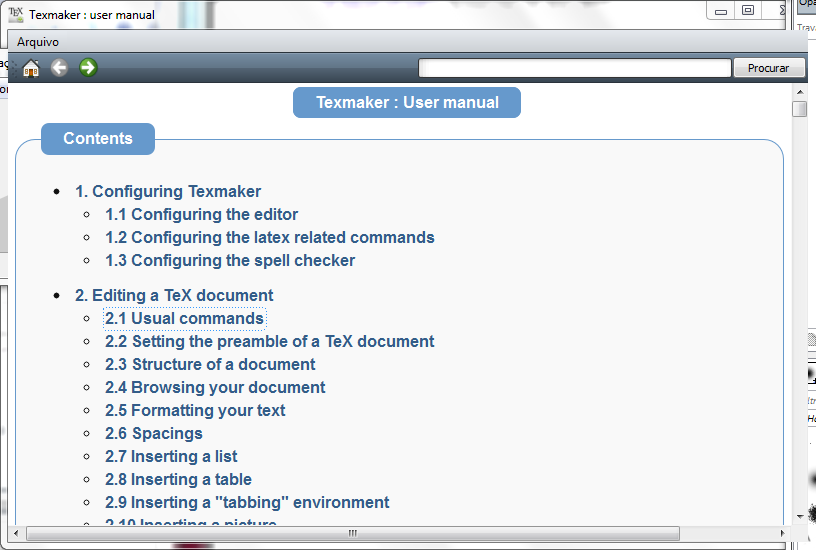
\includegraphics[scale=0.5]
	{img/fig16.png}\label{fig16}\\
	FONTE: Autor (2015)
	\end{figure}

\chapter{Exemplo de apêndice em pdf}
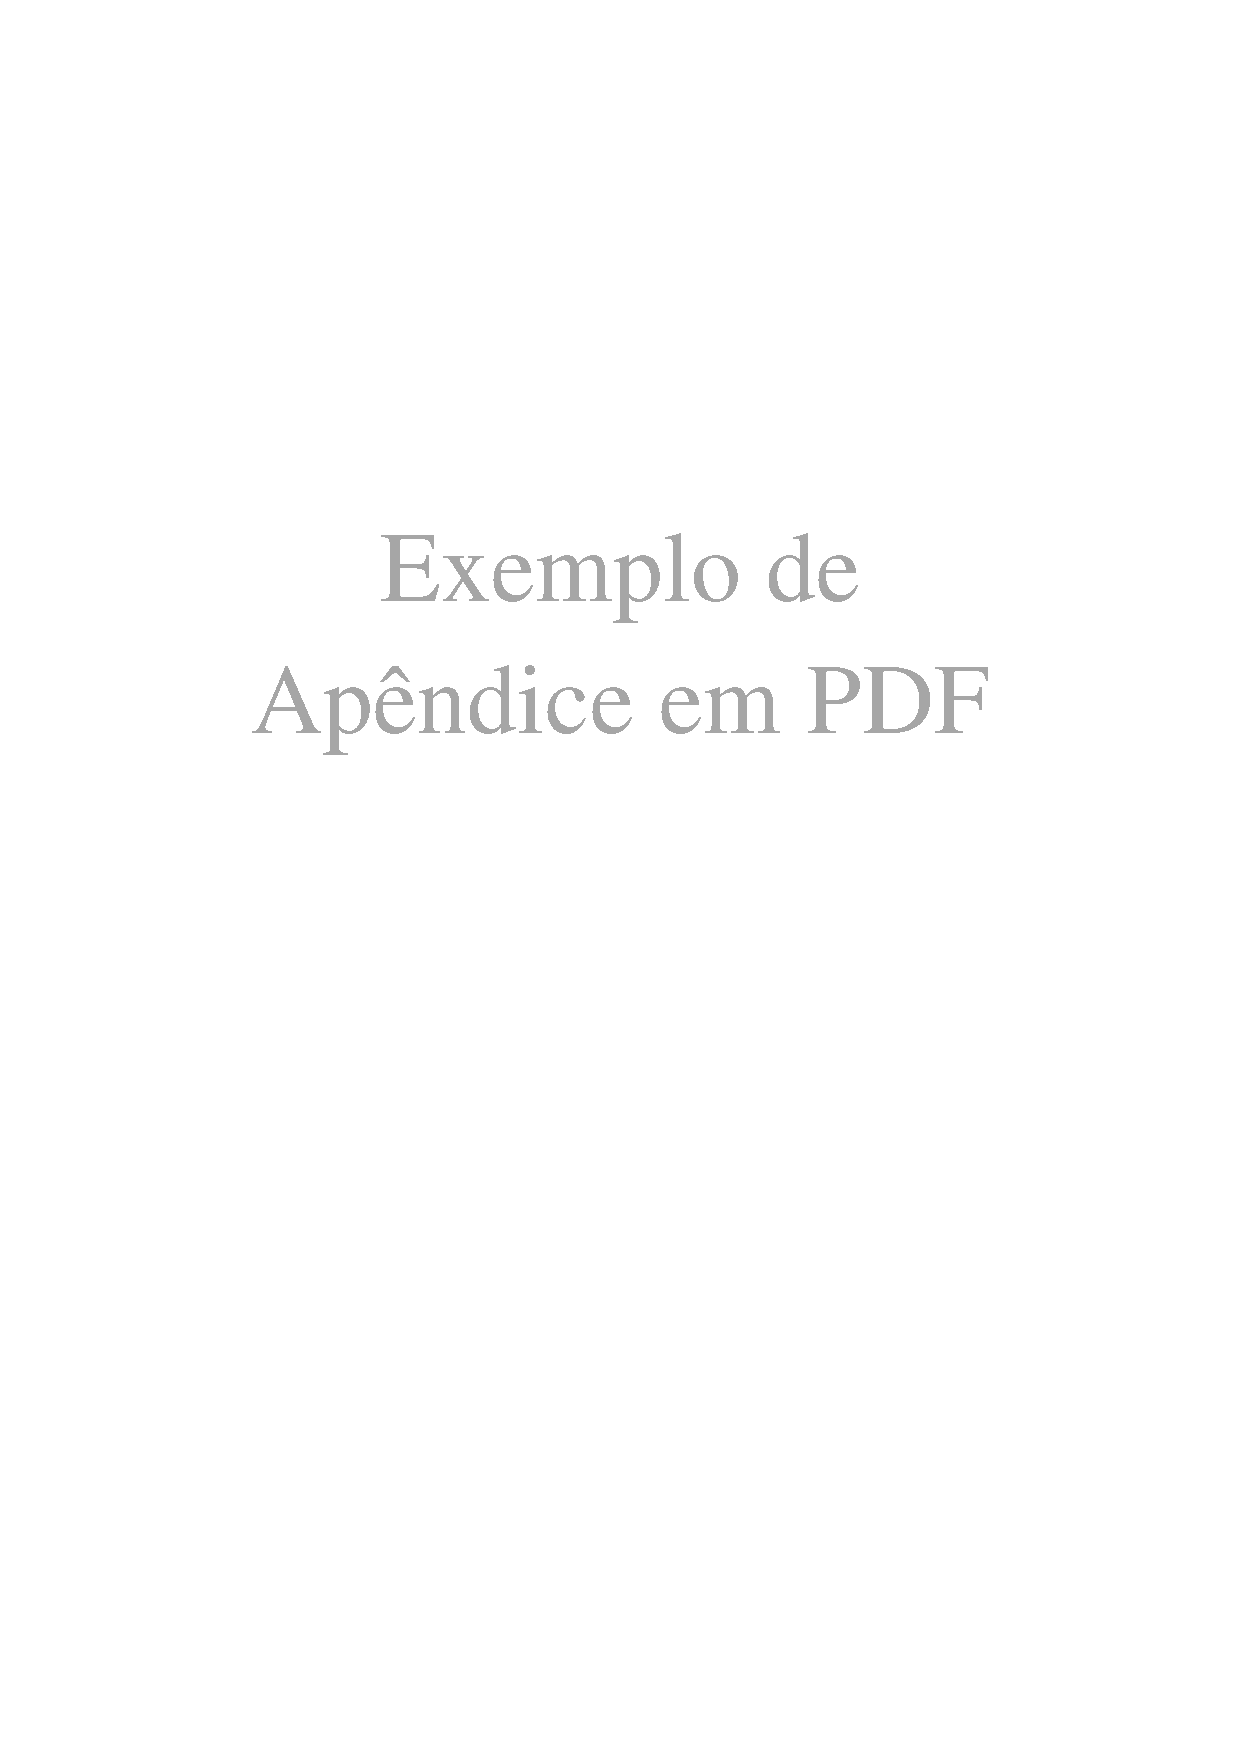
\includepdf[pages=-]{pdf_apendices/apendice_exemplo.pdf}
\end{apendicesenv}

\begin{anexosenv}


%-----------------------------Anexos-----------------------------%
% Imprime uma página indicando o início dos anexos


% ---
\chapter{Exemplo de um anexo digitado}
% ---
\section*{Configuring Texmaker}
Before using Texmaker, you must configure the editor and latex related commands via the ``Configure Texmaker'' command in the ``Options'' menu (``Preferences'' under macosx).
\subsection*{Configuring the editor}

Before compiling your first document, you must set the encoding used by the editor (``Configure Texmaker'' -> ``Editor'' -> ``Editor Font Encoding''). 


% ---
\chapter{Exemplo de anexo em pdf}
% ---
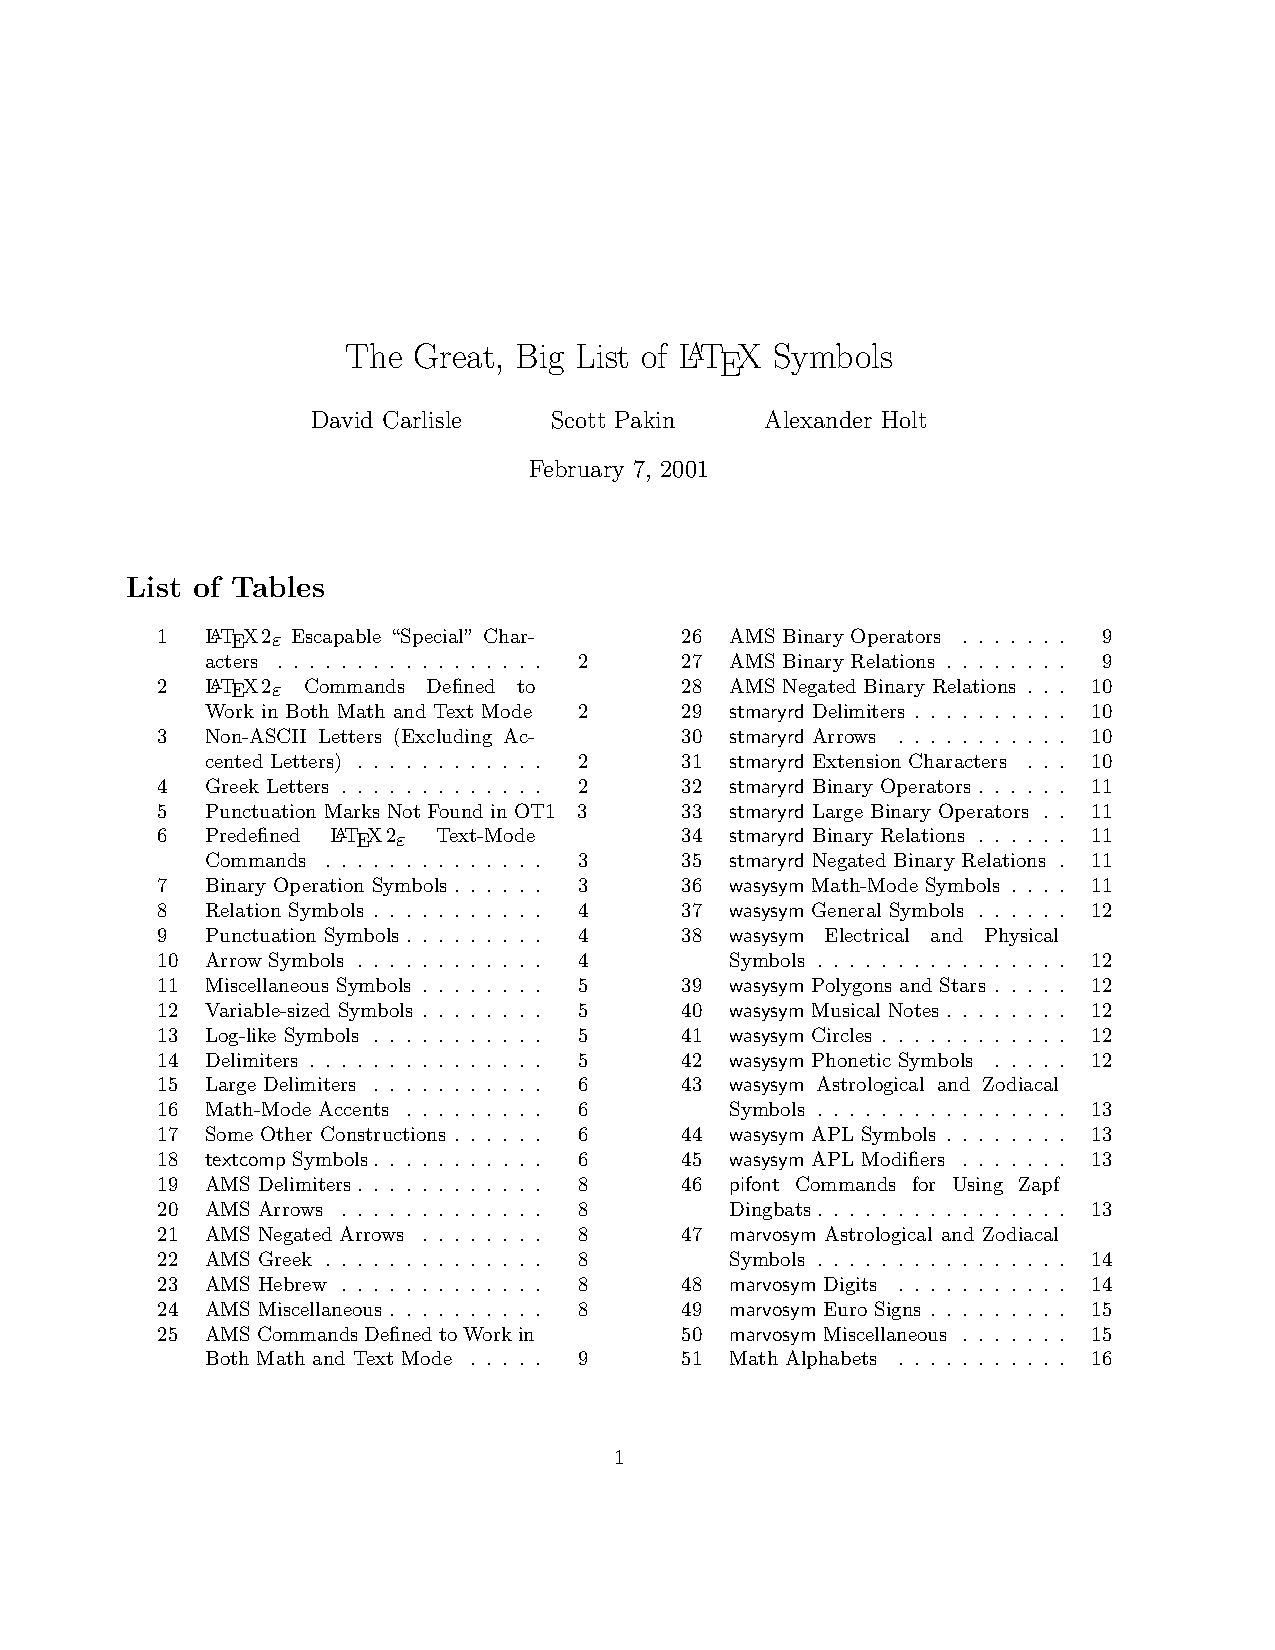
\includepdf[pages=-]{pdf_anexos/anexo_exemplo.pdf}
\end{anexosenv}
